\documentclass{article}

\usepackage[margin=0.5in]{geometry}
\usepackage{multicol}
\usepackage{siunitx}
\usepackage{tikz}
\usepackage{amsthm}

\title{4.3 Solid Geometry Homework}
\author{}
\date{}

\begin{document}
\maketitle

\begin{enumerate}
    \item This figure shows the net of a three-dimensional shape called a truncated octahedron.
        How many vertices does a truncated octahedron have?
        \begin{center}
            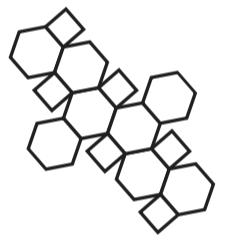
\includegraphics[scale=0.5]{truncated_octahedron.png}
        \end{center}
        \vspace{0.2cm}
    \item What is the greatest distance between any two vertices of a rectangular prism with dimensions $\SI{8}{cm}$ by $\SI{9}{cm}$ by $\SI{12}{cm}$?
        \vspace{3cm}
    \item What is the total surface area of a right square pyramid with a height of $12$ feet and a base with side length of $10$ feet?
        \vspace{3cm}
    \item A right circular cone with base radius $\SI{4}{cm}$ has surface area $\SI{56\pi}{cm^2}$.
        What is the height of the cone?
        Express your answer in simplest radical form.
        \vspace{3cm}
    \item A cylindrical container holds $20$ fluid ounces.
        It has a radius of $3$ inches and a height of $12$ inches.
        How many fluid ounces will a similar container with a radius of $4.5$ inches hold?
        Express your answer as a decimal to the nearest tenth.
        \vspace{3cm}
\end{enumerate}
\end{document}
